\documentclass{article}
\usepackage[main=spanish, provide=*]{babel}
\usepackage{xcolor}
\usepackage{array}
\usepackage{graphicx}
\usepackage{tikz}
\usepackage{circuitikz}
\usepackage{pgfplots}
\usepackage{darkmode}
\usepackage{amsmath}
\usepackage[a4paper, top=2cm, bottom=2cm]{geometry}

\enabledarkmode

\definecolor{c1}{HTML}{8bb6e7}
\definecolor{c2}{HTML}{87f3dd}
\definecolor{c3}{HTML}{fdef83}
\definecolor{c4}{HTML}{fdc373}
\definecolor{c5}{HTML}{fd8581}
\definecolor{c6}{HTML}{c573e7}
\definecolor{c7}{HTML}{afdb68}
\definecolor{c8}{HTML}{e59f8b}

\definecolor{page}{HTML}{262626}
\pagecolor{page}

\renewcommand\thesection{\arabic{part}.\arabic{section}} % Formato de numeración: Parte.Sección
\makeatletter
\@addtoreset{section}{part} % Reinicia el contador de sección con cada parte
\makeatother

\begin{document}
\title{Circuitos trifásicos de corriente alterna sinusoidal}
\author{Mario López Sáez}
\date{\today}
\maketitle

\begin{center}

\begin{tikzpicture}
    \fill[c1] (0, 0) rectangle ++(1, 0.05);
    \fill[c2] (1, 0) rectangle ++(1, 0.05);
    \fill[c3] (2, 0) rectangle ++(1, 0.05);
    \fill[c4] (3, 0) rectangle ++(1, 0.05);
    \fill[c5] (4, 0) rectangle ++(1, 0.05);
    \fill[c6] (5, 0) rectangle ++(1, 0.05);
    \fill[c7] (6, 0) rectangle ++(1, 0.05);
    \fill[c8] (7, 0) rectangle ++(1, 0.05);
\end{tikzpicture}

\end{center}

\part{Generación de 3 fases. Fasores y secuencia. Nomenclatura y concepto de sistema equilibrado de tensiones.}
\section{Generación}


\begin{minipage}{0.49\textwidth}
    \centering
    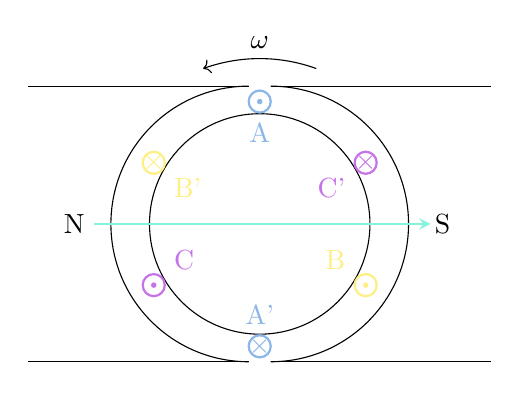
\begin{tikzpicture}[scale=0.7]
        \draw (0, 0) circle (2);
	\draw (-0.2, 2.5) arc [start angle = 90, end angle = 270, radius = 2.5];
	\draw (0.2, -2.5) arc [start angle = -90, end angle = 90, radius = 2.5];
	\draw (-0.2, 2.5) -- ++(-4, 0);
	\draw (-0.2, -2.5) -- ++(-4, 0);
	\draw (0.2, 2.5) -- ++(4, 0);
	\draw (0.2, -2.5) -- ++(4, 0);
	\draw [c1, thick](0, 2.22) coordinate(A) circle (0.2);
	\draw [c1, thick](0, -2.22) coordinate(AA) circle (0.2)node [centered] {$\times$};
	\draw [c3, thick] ({2.22*cos(150)}, {2.22*sin(150)}) coordinate(BB) circle (0.2) node [centered] {$\times$};
	\draw [c6, thick] ({2.22*cos(210)}, {2.22*sin(210)}) coordinate (C) circle (0.2);
	\draw [c6, thick] ({2.22*cos(30)}, {2.22*sin(30)}) coordinate(CC) circle (0.2)node [centered] {$\times$};
	\draw [c3, thick] ({2.22*cos(330)}, {2.22*sin(330)}) coordinate(B) circle (0.2);
        \fill [c1] (A) circle (0.05);
        \fill [c3] (B) circle (0.05);
	\fill [c6] (C) circle (0.05);
	
	\draw [c1] (A |- 0,2) node [below] {A};
	\draw [c1] (AA |- 0,-2) node [above] {A'};
	\draw [c6] (1.73, 1) node [below left] {C'};
	\draw [c6] (-1.73, -1) node [above right] {C};
	\draw [c3] (-1.73, 1) node [below right] {B'};
	\draw [c3] (1.73, -1) node [above left] {B};
	\draw [->, c2, thick, -stealth] (-3, 0) -- (3.1, 0);
	\draw (-3, 0) node [left] {N};
	\draw (3, 0) node [right] {S};
	\draw [->] ({3*cos(70)}, {3*sin(70)}) arc [start angle = 70, end angle = 110, radius = 3];
	\draw (0, 3) node [above] {$\omega$};
    \end{tikzpicture}
\end{minipage}%
\hspace{0.05\textwidth} % Adjust the space between the images if needed
\begin{minipage}{0.45\textwidth}
    \centering
    \begin{circuitikz}[scale=0.8]
        \draw (0, 0.3) to [short, color=c1, o-] ++(0, 0) node [above right] {A'} to [L, color=c1] ++ (0, 3) node [right] {A} to [short, color=c1, -o] ++(0,0) to [open] ++(0, 0.2) node [above] {$AA' \equiv R$};
        \draw (0.3, 0) to [short, color=c3, o-] ++(0, 0) node [below] {B'} to [L, color=c3] ++ (2.6, -1.5) node [right] {B} to [short, color=c3, -o] ++(0,0) to [open] ++(0, -0.2) node [below] {$BB' \equiv S$};
        \draw (-0.3, 0) to [short, color=c6, o-] ++(0, 0) node [above left] {C'} to [L, color=c6] ++ (-2.6, -1.5) node [left] {C} to [short, color=c6, -o] ++(0,0) to [open] ++(0, -0.2) node [below] {$CC' \equiv T$};
    \end{circuitikz}
\end{minipage}

\begin{center}
	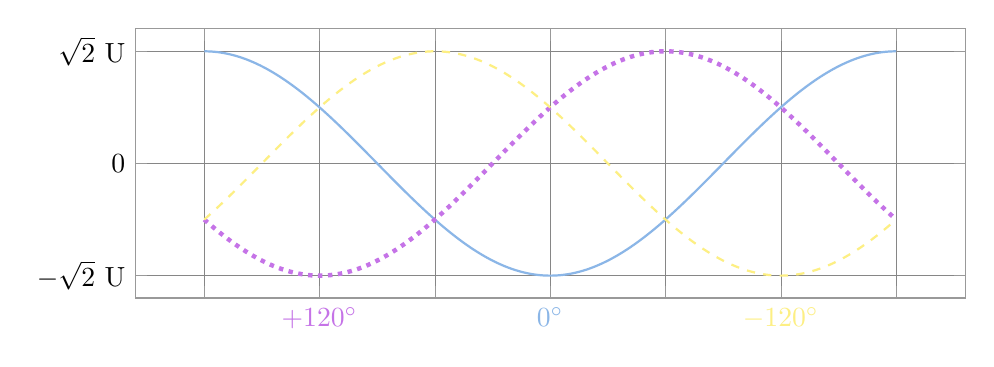
\begin{tikzpicture}
	  	\begin{axis}[
		height=5cm,
		width=\textwidth,
		domain=0:2*pi,
		grid=both,
		yticklabels = {$-\sqrt{2} \text{ U}$, $0$, $\sqrt{2} \text{ U}$}, ytick = {-1, 0, 1},
		xtick = {0, pi/3, 2*pi/3, pi, 4*pi/3, 5*pi/3, 2*pi}, % Los valores en radianes
                xticklabels = {, $\textcolor{c6}{+120^\circ}$, , $\textcolor{c1}{0^\circ}$, , $\textcolor{c3}{-120^\circ}$}, % Etiquetas en grados
		major grid style={line width=.2pt,draw=gray!95},
		samples=100,
		every axis/.append style={axis line style={gray!80}, tick style={gray!80}}
		]
		\addplot[c1, smooth, thick] {cos(deg(x))};
		\addplot[c6, dotted, smooth, ultra thick] {cos(deg(x)+120)};
		\addplot[c3, dashed, smooth, thick] {cos(deg(x)-120)};
		\end{axis}
	\end{tikzpicture}
\end{center}

\section{Nomenclatura}
\begin{flushleft}
$A' \equiv B' \equiv C' \equiv N$ \\

$U_{AA'} = U_{RN}$ ; $U_{BB'} = U_{SN}$ ; $U_{CC'} = U_{TN}$
\end{flushleft}
\begin{center}
    \textbf{FASORES EFICACES}
\end{center}
\[
\begin{array}{rl}
    U_{RN}(t) & = \sqrt{2} U \cos \omega t \hspace{68pt} \underline{U_{RN}} = U \angle 0^\circ \\
    U_{SN}(t) & = \sqrt{2} U \cos (\omega t - 120^\circ) \hspace{30pt} \underline{U_{SN}} = U \angle -120^\circ \\
    U_{TN}(t) & = \sqrt{2} U \cos (\omega t + 120^\circ) \hspace{30pt} \underline{U_{TN}} = U \angle +120^\circ \\
\end{array}
\]
\newpage

\section{Secuencia de fases}
\begin{flushleft}
Hay dos posibilidades en el orden de las señales usando $\underline{U_{AA}}$ como referencia. Una irá $120^\circ$ adelantada, y la otra $120^\circ$ retrasada.
\end{flushleft}
\begin{minipage}{0.48\textwidth}
    \centering
    \hspace{-40pt} \textbf{Secuencia directa} \\[1ex]
    \begin{tikzpicture}[scale=1.2]
        \draw [dashed] (0,0) circle (2);
        \draw [dotted] (0, 0) -- (3.1, 0);
	\draw (3.1, 0) node {\reflectbox{
\includegraphics[width=0.5cm]{ojo.jpg}}};
        \draw [->, c1, thick, -stealth] (0,0) -- +(2,0) node [above right] {$\underline{U}_{AA'}$};
        \draw [->, c6, thick, -stealth] (0,0) -- ({2*cos(120)},{2*sin(120)}) node [above left] {$\underline{U}_{CC'}$}; % 120º
        \draw [->, c3, thick, -stealth] (0,0) -- ({2*cos(240)},{2*sin(240)}) node [below left] {$\underline{U}_{BB'}$}; % 240º
        \draw [<->, latex-latex] (1, 0) arc[start angle = 0, end angle = 120, radius = 1];
        \draw [<->, latex-latex] ({cos(120)},{sin(120)}) arc[start angle=120, end angle=240, radius=1]; % Segundo ángulo
        \draw [<->, latex-latex] ({cos(240)},{sin(240)}) arc[start angle=240, end angle=360, radius=1]; % Tercer ángulo
        \draw ({1.3*cos(60)}, {1.3*sin(60)}) node [centered] {$120^\circ$};
        \draw ({1.4*cos(180)}, 0) node [centered] {$120^\circ$};
        \draw ({1.3*cos(300)}, {1.3*sin(300)}) node [centered] {$120^\circ$};
        \draw [->] ({2.5*cos(30)}, {2.5*sin(30)}) arc[start angle = 30, end angle = 70, radius = 2.5];
        \draw ({2.7*cos(50)}, {2.7*sin(50)}) node [centered] {$\omega$};
        \fill (0, 0) circle (2pt);
    \end{tikzpicture}
\end{minipage}%
\hspace{0.5pt}
\begin{minipage}{0.48\textwidth}
    \centering
    \hspace{-40pt} \textbf{Secuencia inversa} \\[1ex]
    \begin{tikzpicture}[scale=1.2]
        \draw [dashed] (0,0) circle (2);
        \draw [dotted] (0, 0) -- (3.1, 0);
	\draw (3.1, 0) node {\reflectbox{
\includegraphics[width=0.5cm]{ojo.jpg}}};
        \draw [->, c1, thick, -stealth] (0,0) -- +(2,0) node [above right] {$\underline{U}_{AA'}$};
        \draw [->, c3, thick, -stealth] (0,0) -- ({2*cos(120)},{2*sin(120)}) node [above left] {$\underline{U}_{BB'}$}; % 120º
        \draw [->, c6, thick, -stealth] (0,0) -- ({2*cos(240)},{2*sin(240)}) node [below left] {$\underline{U}_{CC'}$}; % 240º
        \draw [<->, latex-latex] (1, 0) arc[start angle = 0, end angle = 120, radius = 1];
        \draw [<->, latex-latex] ({cos(120)},{sin(120)}) arc[start angle=120, end angle=240, radius=1]; % Segundo ángulo
        \draw [<->, latex-latex] ({cos(240)},{sin(240)}) arc[start angle=240, end angle=360, radius=1]; % Tercer ángulo
        \draw ({1.3*cos(60)}, {1.3*sin(60)}) node [centered] {$120^\circ$};
        \draw ({1.4*cos(180)}, 0) node [centered] {$120^\circ$};
        \draw ({1.3*cos(300)}, {1.3*sin(300)}) node [centered] {$120^\circ$};
        \draw [->] ({2.5*cos(30)}, {2.5*sin(30)}) arc[start angle = 30, end angle = 70, radius = 2.5];
        \draw ({2.7*cos(50)}, {2.7*sin(50)}) node [centered] {$\omega$};
        \fill (0, 0) circle (2pt);
    \end{tikzpicture}
\end{minipage}
\\
\begin{flushleft}
Trabajaremos con la secuencia directa
\end{flushleft}

\section{Sistema equilibrado de tensiones}
\begin{flushleft}
Tensiones de igual valor eficaz
\end{flushleft}
$$
U_{RN} = U_{SN} = U_{TN} \hspace{20pt} \to \hspace{20pt} \underline{U_{RN}} + \underline{U_{SN}} + \underline{U_{TN}} = 0 
$$

\begin{flushleft}
Desfasadas $120^\circ$ \\

$\underline{U_{RN}}$, $\underline{U_{SN}}, \underline{U_{TN}}$ Se denominan \textbf{tensiones de fase}
\end{flushleft}
\part{Circuitos a 4 hilos y 3 hilos. Configuraciones $\textsf{Y}$ y $\Delta$. Magnitudes de fase y de línea. Nomenclatura y relaciones $U_{\text{LÍNEA}} \leftrightarrow U_{\text{FASE}}$}

\section{Circuitos a 4 hilos y 3 hilos}

\begin{center}
    
\begin{circuitikz} [scale=0.9]
    \fill (0, 0) coordinate(N) circle (5pt) node [above left] {N};
    \draw (N) to [short] ++(6, 0)node [above left] {N};
    \draw (N) to [vsourcesin, l=$\underline{U_{RN}}$] ++(0, 4) coordinate(R);
    \draw (N) to [vsourcesin, l_=$\underline{U_{SN}}$] ++(3.46, -2) coordinate(S);
    \draw (N) to [vsourcesin, l=$\underline{U_{TN}}$] ++(-3.46, -2) coordinate(T);

    \draw (S) node [above] {S};
    \draw (S) to [short, *-] (6, -2)node [above left] {S};

    
    \draw (T) node [left] {T};
    \draw (T) to [short, *-] ++(0, -2) to [short] (6, -4) node [above left] {T};

    \draw (R) node [above] {R};
    \draw (R) to [short, *-] ++(6, 0)node [above left] {R};

    \draw (6, -5) -- (6, 5) -- (10, 5) -- (10, -5) -- (6, -5);

    \draw [c2] (R) node [below right] {+} to [open, v^<=$\underline{U_{RS}}$] (S);
    \draw [c2] (S|-0,-1.7) node [above left] {$-$};
    \draw [c2] (S) node [below left] {+} to [open, v^<=$\underline{U_{ST}}$] (T) node [right] {$-$};
    \draw [c2] (T) node [above] {+} to [open, v^<=$\underline{U_{TR}}$] (R) node [below left] {$-$};
    \end{circuitikz}

    4 hilos RSTN. 3 hilos RST.
\end{center}
    
\begin{flushleft}
Las tensiones $\underline{U_{RS}}$, $\underline{U_{ST}}$ y $\underline{U_{TR}}$ son \textbf{tensiones de línea}. Se utiliza la permutación positiva de subíndices. $R \to S \to T$ circular. \newline

    Siempre podremos considerar que el sistema de generación está configurado como en el circuito de arriba. Por esta razón, habitualmente no se añadirá la parte de la izquierda, empezando los circuitos desde las 3 o 4 líneas RST(N).
\end{flushleft}

\section{Magnitudes de fase y de línea}
\begin{flushleft}
\textbf{TENSIONES DE FASE O SIMPLES: } $\underline{U_{RN}}$, $\underline{U_{SN}}$, $\underline{U_{TN}}$ \newline
\textbf{TENSIONES DE LÍNEA O COMPUESTAS: } $\underline{U_{RS}}$, $\underline{U_{ST}}$, $\underline{U_{TR}}$
\end{flushleft}
\begin{minipage}{0.45\textwidth}
    \centering
\begin{align*}
    \underline{U_{RS}} & = \underline{U_{RN}} - \underline{U_{SN}} = U \angle 0^\circ - U \angle -120^\circ, \\
    \underline{U_{ST}} & = \underline{U_{SN}} - \underline{U_{TN}} = U \angle -120^\circ - U \angle 120^\circ, \\
    \underline{U_{TR}} & = \underline{U_{TN}} - \underline{U_{RN}} = U \angle 120^\circ - U \angle 0^\circ.
\end{align*}
\begin{align*}
& \text{Mirando la gráfica de la derecha:} \\
& U_{RS}^2 = U^{2} + U^{2} - 2 U U \cos 120^\circ \\
& U_{RS}^2 = 3 U^{2} \\
& U_{RS}  = \sqrt{3} U \\
& \underline{U_{RS}} = \sqrt{3} U \angle 30^\circ = \sqrt{3} \underline{U_{RN}} \angle 30^\circ
\end{align*}
\end{minipage}
\hspace{1cm}
\begin{minipage}{0.45\textwidth}
    \centering
        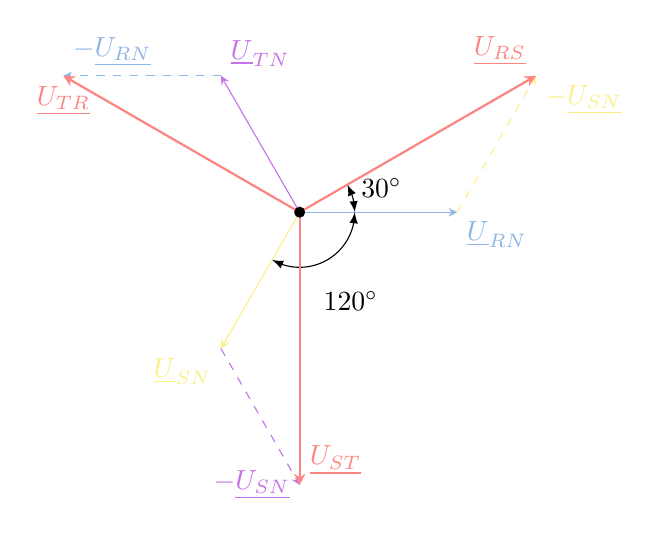
\begin{tikzpicture}[scale=1]
        \draw [->, c1, -stealth] (0,0) -- +(2,0) node [below right] {$\underline{U}_{RN}$} coordinate(RN);
        \draw [->, c6, -stealth] (0,0) -- ({2*cos(120)},{2*sin(120)}) node [above right] {$\underline{U}_{TN}$} coordinate(TN); % 120º
        \draw [->, c3, -stealth] (0,0) -- ({2*cos(240)},{2*sin(240)}) node [below left] {$\underline{U}_{SN}$} coordinate(SN); % 240º
        \draw [<->, latex-latex] (0.7, 0) arc[start angle = 0, end angle = 30, radius = 0.7];
        \draw [<->, latex-latex] ({0.7*cos(240)},{0.7*sin(240)}) arc[start angle=240, end angle=360, radius=0.7]; % Tercer ángulo
        \draw ({1.2*cos(30)}, {1.2*sin(15)}) node [centered] {$30^\circ$};
        \draw ({1.3*cos(300)}, {1.3*sin(300)}) node [centered] {$120^\circ$};
	\draw[->, c3, dashed, -stealth] (RN) -- ++({-2*cos(240)}, {-2*sin(240}) coordinate(NSN) node [below right] {$-\underline{U_{SN}}$};
	\draw[->, c1, dashed, -stealth] (TN) -- ++(-2, 0) coordinate(NRN) node [above right] {$-\underline{U_{RN}}$};
	\draw[->, c6, dashed, -stealth] (SN) -- ++({-2*cos(120)}, {-2*sin(120}) coordinate(NTN) node [left] {$-\underline{U_{SN}}$};
	\draw [->, c5, thick, -stealth] (0, 0) -- (NSN) node [above left] {$\underline{U_{RS}}$};
	\draw [->, c5, thick, -stealth] (0, 0) -- (NRN) node [below] {$\underline{U_{TR}}$};
	\draw [->, c5, thick, -stealth] (0, 0) -- (NTN) node [above right] {$\underline{U_{ST}}$};
        \fill (0, 0) circle (2pt);
    \end{tikzpicture}
\end{minipage}
\textbf{RELACIONES ENTRE TENSIONES DE FASE Y DE LÍNEA PARA TENSIONES EQUILIBRADAS}
$$
\underline{U_{RS}} = \sqrt{3} \underline{U_{RN}} \angle 30^\circ
$$
$$
\underline{U_{ST}} = \sqrt{3} \underline{U_{SN}} \angle 30^\circ
$$
$$
\underline{U_{TR}} = \sqrt{3} \underline{U_{TN} } \angle 30^\circ
$$
$$
\underline{U_{RS}} + \underline{U_{ST}} + \underline{U_{TR}} = 0
$$
\section{Conexiones}

\begin{minipage}{0.45\textwidth}
	\centering
	$$
	\textsf{Y - Y}
	$$
	$$
4 \text{ HILOS } \underline{Z_{N}} \neq \infty ; \ 3 \text{ HILOS } \underline{Z_{N}} \to \infty
	$$
	\resizebox{0.8\textwidth}{!}{
    \begin{circuitikz} [scale=1]
        \draw (0, 0) coordinate(N) circle (4pt) node [above left] {N} to [generic = $\underline{Z_{N}}$, *-] ++(4,0) to [short, -*] ++(2, 0) coordinate(NN) node [right] {N'};
	\draw [c1] (0, 2) coordinate (R) node [above left] {R} to [generic = $\underline{Z_{L}}$, i=$\underline{I_{R}}$, *-] ++(4,0) to [short, -*] ++(2, 0) node [above] {R'} to [generic = $\underline{Z_{R}}$] ++(0, -2);
	\draw [c6] (NN) to [generic, l_= $\underline{Z_{T}}$] ++(-1, -1.73) coordinate(ZT);
	\draw [c6] (0, -4) coordinate (T) node [above left] {T} to [generic = $\underline{Z_{L}}$, i=$\underline{I_{T}}$, *-] ++(4,0) to [short] (ZT |- 0, -4) to [short, -*] (ZT);
	\draw [c3] (NN) to [generic = $\underline{Z_{S}}$] ++(1, -1.73) coordinate(ZS);
	\draw [c3] (0, -2) coordinate (S) node [above left] {S} to [generic = $\underline{Z_{L}}$, i=$\underline{I_{S}}$, *-] ++(4, 0) to [short] (ZS |- 0,-2) to [short, -*] (ZS);
	\draw [c3] (ZS) node [right] {S'};
	\draw [c6] (ZT) node [left] {T'};
    \end{circuitikz}
}
\end{minipage}
\begin{minipage}{0.45\textwidth}
	\centering
	$$
	\textsf{Y} - \Delta
	$$
	$$
3 \text{ HILOS } 
	$$
	\resizebox{0.8\textwidth}{!}{
	\begin{circuitikz} [scale=1]
	\draw [c1] (0, 2) coordinate (R) node [above left] {R} to [generic = $\underline{Z_{L}}$, i=$\underline{I_{R}}$, *-] ++(4,0) to [short, -*] ++(2, 0) node [above] {R'} coordinate(RR);
	\draw (RR) to [generic = $\underline{Z_{TR}}$, i_<=$\underline{I_{\text{T'R'}}}$] ++(-2, -3.46) coordinate(TT) to [generic = $\underline{Z_{ST}}$, i_<=$\underline{I_{\text{S'T'}}}$] ++(4, 0)   coordinate(SS) to [generic = $\underline{Z_{RS}}$, i_<=$\underline{I_{\text{R'S'}}}$] (RR);
	\draw [c6] (0, -4) coordinate (T) node [above left] {T} to [generic = $\underline{Z_{L}}$, i=$\underline{I_{T}}$, *-] ++(4,0) to [short] (TT |- 0, -4) to [short, -*] (TT);
	\draw [c3] (0, -2) coordinate (S) node [above left] {S} to [generic = $\underline{Z_{L}}$, i=$\underline{I_{S}}$, *-] ++(4, 0) to [short] (SS |- 0,-2) to [short, -*] (SS);
	\draw [c3] (SS) node [right] {S'};
	\draw [c6] (TT) node [left] {T'};
    \end{circuitikz}
}
\end{minipage}
\begin{flushleft}
En la configuración estrella - estrella, las corrientes de línea y las de fase coinciden. Sin embargo, las tensiones de fase y de línea no. \newline

En la cofiguración triángulo - estrella, las corrientes de línea y las de fase son iguales en generación, pero diferentes en recepción. Sin embargo, aquí las tensiones de fase y de línea son $\text{U}_{\text{R'S'}}$, $\text{U}_{\text{S'T'}}$ y $\text{U}_{\text{T'R'}}$ \newline

$\underline{Z_{L}}$ es el fasor de impedancia de línea, en principio igual. Es la impedancia del propio medio, por lo que, en caso de considerar un medio ideal, no estarían.
\end{flushleft}

\part{Teorema de Millman. Análisis de circuitos generales}
\section{Teorema de Millman}
\begin{flushleft}
En un circuito eléctrico de ramas en paralelo, cada una compuesta por una fuente de tensión ideal en serie con un elemento lineal, la tensión en los terminales de las ramas es igual a la suma de las fuerzas electromotrices multiplicadas por la admitancia de la rama dividido por la suma de las admitancias. - Jacob Millman
\end{flushleft}
\begin{minipage}{0.45\textwidth}
	\centering
\resizebox{1\textwidth}{!}{
\begin{circuitikz} [american]

\foreach \x [count=\n from 1] in {0, 2, 4} {
    \draw (\x, 0) 
        to [generic=$\underline{Z_{\n}}$, i^=$\underline{I_{\n}}$, c5, color=c5, -o] ++(0, -3) 
        to [open, v=$U_{\n B}$, c2, color=c2] ++(0, -2) 
        to [short, o-] ++(0, -1);
}

\draw (8, 0) to [generic=$\underline{Z_{N}}$, i^=$\underline{I_{N}}$, -o] ++(0, -3) to [open, v=$U_{NB}$, c2, color=c2] ++(0, -2) to [short, o-] ++(0, -1);

\draw (0,0) to [short, -o] ++(10, 0) node [above] {A};
\draw (0,-6) to [short, -o] ++(10, 0) node [below] {B};
\draw (10, 0) to [open, v=$U_{\text{AB}}$] (10, -6);
\draw [->] (9.5, 0.3) -- ++(-1, 0) node [above right] {$\underline{I} = 0$};
\fill (5.7, -3) circle (0.05) ++(0.3, 0) circle (0.05) ++(0.3, 0) circle (0.05);
\end{circuitikz}
}
\end{minipage}
\begin{minipage}{0.5\textwidth}
	\centering
    \begin{align*}
	& \sum \underline{I_{i}} = 0 \\
	& \underline{I_{1}} = \frac{\underline{U_{AB}} - \underline{U_{1B}}}{Z_{1}} \\
	& \cdot \\
	& \cdot \\
	& \cdot \\
	& \underline{I_{N}} = \frac{\underline{U_{AB}} - \underline{U_{NB}}}{Z_{N}}
    \end{align*}
\end{minipage}

\begin{equation}
	\Large
\underline{U_{\text{AB}}} = \frac{\frac{\underline{U_{\text{1B}}}}{\underline{Z_{1}}}+ \frac{\underline{U_{\text{2B}}}}{\underline{Z_{2}}}+\cdot \cdot \cdot + \frac{\underline{U_{\text{NB}}}}{\underline{Z_{N}}}}{\frac{1}{\underline{Z_{1}}}+\frac{1}{\underline{Z_{2}}}+ \cdot \cdot \cdot + \frac{1}{\underline{Z_{N}}}}
\end{equation}
\section{Análisis del caso general $\textsf{Y - Y}$}
\begin{center}
    
	\resizebox{0.8\textwidth}{!}{
    \begin{circuitikz} [thick, scale=1]
	    \fill (0, 0) coordinate(N) circle (5pt) node [above left] {N};
	    \draw[c2!50] (N) to [vsourcesin, l=$\underline{U_{RN}}$] ++(0, 4) coordinate(R);
	    \draw[c2!200] (N) to [vsourcesin, l_=$\underline{U_{SN}}$] ++(3.46, -2) coordinate(S);
	    \draw[c2] (N) to [vsourcesin, l=$\underline{U_{TN}}$] ++(-3.46, -2) coordinate(T);

        \draw (N) circle (4pt) node [above left] {N} to [generic = $\underline{Z_{N}}$, *-] ++(6,0) coordinate(NN) node [right] {N'};
	\draw [c5!70] (R) node [above left] {R} to [generic = $\underline{Z_{L}}$, i=$\underline{I_{R}}$, *-] ++(6, 0) node [above] {R'} to [short] ++(0,-1) to [generic = $\underline{Z_{R}}$] (NN);
	\draw [c5!120] (NN) to [generic, l_= $\underline{Z_{T}}$] ++(-2, -3.46) coordinate(ZT);
	\draw [c5!120] (T) to [short] ++(0, -3) node [above left] {T} to [generic = $\underline{Z_{L}}$, i=$\underline{I_{T}}$, *-] (ZT |- 0, -5) to [short, -*] (ZT);
	\draw [c5!160] (NN) to [generic = $\underline{Z_{S}}$] ++(2, -3.46) coordinate(ZS);
	\draw [c5!160] (S) to [short] ++(0, -2) node [above left] {S} to [generic = $\underline{Z_{L}}$, i=$\underline{I_{S}}$, *-] ++(4, 0) to [short] (ZS |- 0,-4) to [short, -*] (ZS);
	\draw [c5] (ZS) node [right] {S'};
	\draw [c5] (ZT) node [left] {T'};
    \end{circuitikz}
}
\end{center}
\begin{center}
Analizamos la malla N $\to$ R $\to$ R' $\to$ N' $\to$ N
\end{center}
$$
\underline{U_{\text{RN}}} - \underline{I_{R}} \underline{Z_{L}} - \underline{I_{R}} \underline{Z_{R}}- \underline{U_{\text{N'N}}} 
$$
\begin{center}
Conociendo $\underline{U_{\text{N'N}}}$ podemos calcular el resto de valores.
\end{center}
$$
\underline{I_{R}} = \frac{\underline{U_{\text{RN}}} - U_{\text{N'N}}}{\underline{Z_{L}} + \underline{Z_{R}}}; \ \underline{I_{S}} = \frac{\underline{U_{\text{SN}}} - U_{\text{N'N}}}{\underline{Z_{L}} + \underline{Z_{S}}}; \ \underline{I_{T}} = \frac{\underline{U_{\text{TN}}} - U_{\text{N'N}}}{\underline{Z_{L}} + \underline{Z_{T}}}
$$

\begin{equation}
    \Large
    \underline{U_{\text{N'N}}} = \frac{    \frac{\underline{U_{\text{RN}}}}{\underline{Z_{L}} + \underline{Z_{R}}} +
    \frac{\underline{U_{\text{SN}}}}{\underline{Z_{L}} + \underline{Z_{S}}} +
    \frac{\underline{U_{\text{TN}}}}{\underline{Z_{L}} + \underline{Z_{T}}} +
    \frac{0}{\underline{Z_{N}}} }{\frac{1}{\underline{Z_{L} + Z_{R}}} + \frac{1}{\underline{Z_{L} + Z_{S}}} + \frac{1}{\underline{Z_{L} + Z_{T}}} + \frac{1}{\underline{Z_{N}}}}
\end{equation}


\part{Potencia trifásica y corrección del factor de potencia}
\section{Potencia trifásica en sistemas equilibrados}
\begin{table}[h!]
\centering
\begin{tabular}{c c c}
    $\underline{U_{\text{RN}}}$ & $\underline{U_{\text{SN}}}$ & $\underline{U_{\text{TN}}}$ \\
    $U \angle 0^\circ$ & $U \angle -120^\circ$ & $U \angle 120^\circ$ \\
    $\underline{I_{R}}$ & $\underline{I_{S}}$ & $\underline{I_{T}}$ \\
    $I \angle - \varphi$ & $I \angle - \varphi - 120^\circ$ & $I \angle - \varphi + 120^\circ$ \\
\end{tabular}
\label{tabla:pot}
\end{table}

\subsection{Potencia instantánea constante}
\begin{align*}
	p_{R} (t) & = UI \cos \varphi + UI \cos (2 \omega t - \varphi) \\
	+ \ p_{S} (t) & = UI \cos \varphi + UI \cos (2 \omega t - \varphi - 120^\circ) \\
	p_{T} (t) & = UI \cos \varphi + UI \cos (2 \omega t - \varphi + 120^\circ) 
\end{align*}
\hline

$$
p_{TOTAL} (t) = 3 UI \cos \varphi + 0 \to \text{CONSTANTE}
$$



\part{Ventajas de los sistemas trifásicos}
\begin{flushleft}
1. Más económico que el monofásico. A una tensión e igualdad de potencia a transmitir e igualdad de pérdidas en la línea, el ahorro en el cobre es de un $25\%$ \newline

2. La potencia instantánea trifásica es constante, independiente del tiempo, por ello los motores trifásicos tienen un par uniforme, evitando vibraciones y esfuerzos en el rotor. \newline

3. Los motores trifásicos pueden arrancar por sí mismos. Sin embargo, los motores monofásicos necesitan dispositivos especiales para conseguir su arranque.
\end{flushleft}
\begin{minipage}{0.45\textwidth}
	\centering
	\begin{circuitikz}[american]
	    \draw (0, 0) to [short, i=$I_{1}$,*-] ++(3,0);
	    \draw (0, -2) to [short, *-] ++(3,0);
	    \draw (0, 0) to [open, v=$U$] ++(0, -2);
	    \draw [->] (3.1, 0.2) -- (3.1, -0.2) -- ++(0.3, 0) node [right] {$\text{P}_{\text{M}}$};
	\end{circuitikz}
	$$
P_{M} = U I_{1} \cos \varphi
	$$
	$$
P_{\text{LÍNEA}} = 2 R_{1} I_{1}^2
	$$
	$$
R_{1} = \rho \cdot \frac{L}{S_{1}}
	$$
    
\end{minipage}
\hspace{0.05pt}
\begin{minipage}{0.45\textwidth}
	\centering
	\begin{circuitikz}[american]
	    \draw (0, 0) to [short, i=$I_{3}$,*-] ++(3,0);
	    \draw (0, -1) to [short, *-] ++(3,0);
	    \draw (0, -2) to [short, *-] ++(3,0);
	    \draw (-0.5, 0.15) to [open, v=$U$] ++(0, -1.35);
	    \draw [->] (3.1, 0.2) -- (3.1, -0.2) -- ++(0.3, 0) node [right] {$\text{P}_{\text{T}}$};
	\end{circuitikz}
	$$
P_{T} = \sqrt{3} \ U I_{3} \cos \varphi
	$$
	$$
P_{\text{LÍNEA}} = 3 R_{3} I_{3}^2
	$$
	$$
R_{3} = \rho \cdot \frac{L}{S_{3}}
	$$
    
\end{minipage}
$$
P_{M} = P_{T}
$$
$$
\frac{\text{PESO COBRE TRIFÁS.}}{\text{PESO COBRE MONO.}} = \frac{3}{4}
$$
\end{document}
